
%%%%%%%% ICML 2026 EXAMPLE LATEX SUBMISSION FILE %%%%%%%%%%%%%%%%%

\documentclass{article}

% Recommended, but optional, packages for figures and better typesetting:
\usepackage{microtype}
\usepackage{graphicx}
\usepackage{subcaption}
\usepackage{booktabs} % for professional tables
\usepackage{multirow}
\usepackage{makecell}
% hyperref makes hyperlinks in the resulting PDF.
% If your build breaks (sometimes temporarily if a hyperlink spans a page)
% please comment out the following usepackage line and replace
% \usepackage{icml2026} with \usepackage[nohyperref]{icml2026} above.
\usepackage{hyperref}
\usepackage{siunitx}
\usepackage{booktabs}
\usepackage{multirow}
\usepackage{siunitx}
\usepackage{float}

\usepackage{tikz}
  \usetikzlibrary{arrows.meta,positioning}
  
\sisetup{
  detect-weight=true,
  table-number-alignment=center,
  round-mode=places,
  round-precision=4
}

% Attempt to make hyperref and algorithmic work together better:
\newcommand{\theHalgorithm}{\arabic{algorithm}}

% Use the following line for the initial blind version submitted for review:
\usepackage{icml2026}

% For preprint, use
% \usepackage[preprint]{icml2026}

% If accepted, instead use the following line for the camera-ready submission:
% \usepackage[accepted]{icml2026}

\usepackage{amsmath}
\usepackage{amssymb}
\usepackage{mathtools}
\usepackage{amsthm}


% if you use cleveref..
\usepackage[capitalize,noabbrev]{cleveref}

%%%%%%%%%%%%%%%%%%%%%%%%%%%%%%%%
% THEOREMS
%%%%%%%%%%%%%%%%%%%%%%%%%%%%%%%%
\theoremstyle{plain}
\newtheorem{theorem}{Theorem}[section]
\newtheorem{proposition}[theorem]{Proposition}
\newtheorem{lemma}[theorem]{Lemma}
\newtheorem{corollary}[theorem]{Corollary}
\theoremstyle{definition}
\newtheorem{definition}[theorem]{Definition}
\newtheorem{assumption}[theorem]{Assumption}
\theoremstyle{remark}
\newtheorem{remark}[theorem]{Remark}

% Todonotes is useful during development; simply uncomment the next line
%    and comment out the line below the next line to turn off comments
%\usepackage[disable,textsize=tiny]{todonotes}
\usepackage[textsize=tiny]{todonotes}

% The \icmltitle you define below is probably too long as a header.
% Therefore, a short form for the running title is supplied here:
\icmltitlerunning{PP-Mark: Provable and Publicly Verifiable Watermarking for Generative AI}

\begin{document}

\twocolumn[
  \icmltitle{PP-Mark: Provable and Publicly Verifiable Watermarking for Generative AI}

  % It is OKAY to include author information, even for blind submissions: the
  % style file will automatically remove it for you unless you've provided
  % the [accepted] option to the icml2026 package.

  % List of affiliations: The first argument should be a (short) identifier you
  % will use later to specify author affiliations Academic affiliations
  % should list Department, University, City, Region, Country Industry
  % affiliations should list Company, City, Region, Country

  % You can specify symbols, otherwise they are numbered in order. Ideally, you
  % should not use this facility. Affiliations will be numbered in order of
  % appearance and this is the preferred way.
  \icmlsetsymbol{equal}{*}

  \begin{icmlauthorlist}
    \icmlauthor{}{}
    \icmlauthor{Firstname2 Lastname2}{equal,yyy,comp}
    \icmlauthor{Firstname3 Lastname3}{comp}
    \icmlauthor{Firstname4 Lastname4}{sch}
    \icmlauthor{Firstname5 Lastname5}{yyy}
    \icmlauthor{Firstname6 Lastname6}{sch,yyy,comp}
    \icmlauthor{Firstname7 Lastname7}{comp}
    %\icmlauthor{}{sch}
    \icmlauthor{Firstname8 Lastname8}{sch}
    \icmlauthor{Firstname8 Lastname8}{yyy,comp}
    %\icmlauthor{}{sch}
    %\icmlauthor{}{sch}
  \end{icmlauthorlist}

  \icmlaffiliation{yyy}{Department of XXX, University of YYY, Location, Country}
  \icmlaffiliation{comp}{Company Name, Location, Country}
  \icmlaffiliation{sch}{School of ZZZ, Institute of WWW, Location, Country}

  \icmlcorrespondingauthor{}{}
  \icmlcorrespondingauthor{}{}

  % You may provide any keywords that you find helpful for describing your
  % paper; these are used to populate the "keywords" metadata in the PDF but
  % will not be shown in the document
  \icmlkeywords{Machine Learning, ICML}

  \vskip 0.3in
]

% this must go after the closing bracket ] following \twocolumn[ ...

% This command actually creates the footnote in the first column listing the
% affiliations and the copyright notice. The command takes one argument, which
% is text to display at the start of the footnote. The \icmlEqualContribution
% command is standard text for equal contribution. Remove it (just {}) if you
% do not need this facility.

% Use ONE of the following lines. DO NOT remove the command.
% If you have no special notice, KEEP empty braces:
\printAffiliationsAndNotice{}  % no special notice (required even if empty)
% Or, if applicable, use the standard equal contribution text:
% \printAffiliationsAndNotice{\icmlEqualContribution}

\begin{abstract} 
Generative AI models now produce images that are difficult to distinguish from real data, making publicly verifiable provenance essential; however, existing invisible and semantic watermarking methods become vulnerable to black-box imprint forgeries and adaptive optimization attacks once their detectors are made public. We propose PP-Mark, a provenance framework that achieves unforgeability and public verifiability by binding statistical watermark detection to cryptographic commitments. PP-Mark enforces consistency between the generation context and image-specific latent traces using zero-knowledge proofs, thereby preventing adversarial optimization against the detector, and ensuring that forged content fails verification by construction. Experimental results show that PP-Mark is robust to advanced forgery attacks while remaining computationally efficient for decentralized verification.
\end{abstract}


\section{Introduction}
The rapid proliferation of generative AI has fundamentally challenged our ability to distinguish between human-authored and machine-generated media. As synthetic content becomes increasingly indistinguishable from reality, it facilitates the spread of deepfakes, coordinated disinformation, and large-scale digital forgery \cite{chesney_citron2019}. This shift has created an urgent societal and regulatory demand for verifiable provenance, requiring AI systems to provide reliable evidence of machine origin that can be independently audited by the public \cite{longpre2024dataauth}. In response, industry-wide initiatives such as the C2PA (Coalition for Content Provenance and Authenticity) and regulatory frameworks including the EU AI Act have emerged, mandating explicit identification and labeling of AI-generated content \cite{c2pa_spec_2_3}. Ultimately, the effectiveness of these standards depends critically on the robustness of the underlying technical mechanisms used to attest to content origin.

Digital watermarking has emerged as a promising approach for establishing robust provenance of generative content. Conventional post-hoc invisible watermarking methods embed signals in the pixel or frequency domain after image generation (e.g., \cite{zhu2018hidden}). Although such techniques largely preserve visual quality, they remain vulnerable to regeneration, denoising, and other model-based attacks that can remove or attenuate the embedded signal \cite{zhao2024removable}. To mitigate these weaknesses, recent work has shifted toward semantic watermarking, which injects structured signals directly into the latent space or the denoising trajectory during the generative process \cite{wen2023treerings,fernandez2023stablesignature,zhang2024zodiac}. By entangling the watermark with the semantic structure of the image, methods such as Tree-Rings \cite{wen2023treerings} exhibit improved robustness against low-level image manipulations.

Despite these advances, we identify a fundamental and previously overlooked vulnerability in existing semantic watermarking schemes. First, recent black-box imprint forgery attacks demonstrate that an adversary, given access to only a single watermarked reference image, can extract and hallucinate watermark patterns into forged images by minimizing distances in the latent space \cite{muller2025blackbox}. Second, a more severe optimization vulnerability emerges when watermark detectors $D(\cdot)$ are made public. In this setting, the detector effectively functions as a differentiable or queryable loss, enabling adversaries to iteratively optimize forged content to satisfy the verification criterion itself, rather than merely transferring watermark patterns \cite{jiang2023evading}. More broadly, recent studies show that public exposure of detection components and auxiliary signals can substantially weaken semantic watermarking pipelines, enabling surrogate-based optimization attacks that exceed the assumptions of conventional threat models \cite{lin2025crack}.

To mitigate these forgery risks, existing systems often rely on centralized verification, keeping the detector $D(\cdot)$ private and exposing it only through permissioned APIs. Although this approach prevents direct leakage of the detection rule as a differentiable or queryable loss function, it introduces a persistent trust bottleneck by preventing independent public auditing of provenance claims. Such centralization turns the verifier into a single point of both technical and institutional failure, effectively converting verification into a costly, permissioned service rather than a transparent public utility. As a result, the field faces a fundamental tension between private verification, which sacrifices public auditability, and public verification, which remains vulnerable to adversarial optimization. Recent work on privacy-preserving verification reflects this same tension by seeking to enable ownership or authenticity checks without revealing sensitive watermarking information \cite{guo2024zeromark}.

In this paper, we resolve this tension by introducing PP-Mark (Provable Presence Mark), a provenance framework for AI-generated content that is both publicly verifiable and resistant to forgery. Our key insight is to reformulate verification from a purely statistical inference problem into a cryptographically grounded proof. Rather than relying solely on a public detection score, which can be reverse-engineered or optimized against, PP-Mark anchors the verification rule to the specific generation context using zero-knowledge proofs (ZKP), ensuring that successful verification requires cryptographic consistency rather than detector manipulation.

By requiring a valid zero-knowledge proof bound to a unique commitment root, PP-Mark ties the statistical detection rule to cryptographic consistency. Our empirical evaluation shows that PP-Mark is more robust than existing baselines under forgery attacks, while the associated cryptographic proofs remain strictly non-transferable to forged content. Because generating a new valid proof is computationally infeasible without access to the generator’s secret witness, PP-Mark enables decentralized and open verification using only public artifacts, while preventing the verification rule itself from being exploited for adversarial forgery.

We summarize our contributions as follows.
\begin{itemize}
    \item We introduce a forgery-resistant public verification mechanism that cryptographically anchors the detection rule, preventing adversarial optimization for forgery.
    \item We propose a context-bound latent embedding scheme that deterministically binds watermark signals to the generation context, ensuring non-transferability across images and preventing reuse without cryptographic detection.
    \item We design a decentralized zero-knowledge verification framework based on SP1 that enables standalone public verification without reliance on centralized APIs.
\end{itemize}
  
\section{Related Works} 
\subsection{From Post-hoc to Robust Semantic Watermarking} 
Early invisible watermarking mostly relied on post-hoc domain injections, such as HiDDeN and StegaStamp \cite{zhu2018hidden,tancik2020stegastamp}, which remain inherently fragile to model-based regenerations. To address this, semantic watermarking entangles the signal with the generative process, as seen in Tree-Rings \cite{wen2023treerings}. Recent robustness-oriented baselines further strengthen semantic marks: DiffuseTrace \cite{lei2024diffusetrace} introduces inversion-aware training with a learned encoder--decoder for robust extraction, while Fourier-integrity variants such as SFW enforce Hermitian symmetry in the latent Fourier domain to improve robustness and fidelity \cite{lee2025iccv_sfw}. While these methods achieve high detection rates under aggressive manipulations, they primarily target traceability under privileged access, leaving a gap in preventing model-based forgery attacks.

\subsection{Large-Scale Identification and Scalable Retrieval}
RingID \cite{ci2024ringid} introduces multi-key identification for better separability. In parallel, WIND proposes a scalable two-stage public detection pipeline that first retrieves a coarse group identifier and then performs within-group search over a large key space \cite{arabi2025wind}. Similarly, MaXsive and TraceMark-LDM target high-capacity identification at scale with robustness to geometric transforms and regeneration, pushing capacity and robustness through initial-noise watermarking and robust attribution mechanisms \cite{luo2025tracemarkldm,mao2025maxsive}. However, these retrieval-based designs primarily optimize identification throughput and operating practicality. They remain vulnerable to forgery and replay attacks that exploit exposed detection oracles \cite{jiang2023evading,muller2025blackbox}.

\subsection{Cryptographic Binding and Secure Public Verification}
The need for secure public verification has led to a transition toward hybrid cryptographic schemes. A conceptual parallel is found in VeriLLM \cite{wang2025verillm}, which uses sampling-based commitments and randomized openings to enable publicly verifiable checking with sublinear overhead. Inspired by this, PP-Mark bridges semantic watermarking and cryptographic unforgeability. PP-Mark enforces a rigorous binding between the image hash and randomized latent openings. This ensures that any adversarial modification results in a cryptographic verification failure, effectively mitigating the forgery risks inherent in modern latent diffusion models. 


  \begin{figure*}[t]
    \centering
    \includegraphics[width=\textwidth]{Approach2.pdf}
    \caption{PP-Mark overview. The generator embeds a latent watermark, commits sampled traces to a Merkle root, and produces an ZKP receipt. Verification uses latent inversion to compute a detection score and validates the receipt; acceptance requires both.}
    \label{fig:overview}
  \end{figure*}
  
\section{Method}
PP-Mark binds a latent-space watermark to the generation context and attaches a standalone SP1 zero-knowledge proof \cite{succinct2024sp1}. Provenance can be verified by any third party using only public artifacts, through a combination of a detection score and cryptographic proof verification.

\subsection{Overview and Threat Model}
We assume an adversary with access to watermarked images and public artifacts, who can perform arbitrary image manipulations. The adversary may attempt black-box imprint forgery or watermark removal attacks. However, the adversary does not possess the secret key and is assumed incapable of forging zero-knowledge proof receipts or breaking standard cryptographic hash functions.

PP-Mark aims to (i) enable public, decentralized provenance verification without proprietary decoders or APIs, (ii) keep the binding key private while allowing third parties to verify correctness, (iii) prevent reuse or transfer by binding each watermark to the generation context, and (iv) maintain detectability under common transformations using a calibrated threshold \(\tau\) that controls false positives. Verification consists of two checks: watermark detection via a correlation score compared against \(\tau\), and validation of a ZKP receipt.

On the generation side, PP-Mark embeds a spread-spectrum watermark into the initial latent noise, commits sampled traces into a Merkle root \cite{merkle87}, and produces a ZKP receipt proving consistency between the binding and the commitment. The resulting metadata includes the context hash \(h_{\mathrm{ctx}}\), binding value \(b\), commitment root \(\mathrm{sample\_root}\), and audit parameters such as \(N\), \(\alpha_{\mathrm{eff}}\), the model identifier, and the LUT hash. The sample trace itself remains private and serves only as a proof witness.

On the verification side, a verifier performs latent inversion from the image, reconstructs the expected watermark signs from the public binding value \(b\), computes the detection score, and validates the ZKP receipt using public inputs. Because verification relies exclusively on public artifacts, PP-Mark enables decentralized provenance checks without proprietary decoders or centralized APIs, while the cryptographic proof prevents the verification rule from being exploited for forgery; the secret key never leaves the generator, yet any third party can independently verify provenance.

\subsection{Notation}
The generation context consists of a prompt $p$, random seed $s$, and model identifier $M$, with secret key $k$. The context hash is denoted by $h_{\mathrm{ctx}}$, and the corresponding public binding value by $b$. The truncated message is $m$, encoded as a Reed–Solomon codeword $c$ and expanded into a bitstream $\mathtt{bits}$. The latent grid is $Z \in \mathbb{R}^{H \times W \times 4}$, indexed by $i$ or equivalently $(x,y,\mathrm{ch})$. The inverse-CDF lookup table is $F^{-1}$. A deterministic sample set $S$ of size $|S|=N$ is used for watermark embedding. For each sampled index, $g_i$ denotes the Gaussian baseline and $z_i$ the corresponding watermarked latent. We denote the normalized initial latent as $z^{(0)}$, and the latent recovered via DDIM inversion as $\hat{z}^{(0)}$. The effective watermark strength is $\alpha_{\mathrm{eff}}$.

For provenance verification, $s_i \in {-1,+1}$ denotes the expected sign pattern and $r_i$ the recovered residual. The sampled trace is denoted by $\mathcal{T}$ and committed to the Merkle root $\mathrm{sample_root}$. The final detection score is $\mathrm{score}$ with threshold $\tau$, and the SP1 zero-knowledge proof receipt is denoted by $\pi$. We define a normalized image hash $h_{\mathrm{img}}$ derived according to a fixed hash specification. The opening challenge seed is defined as
$\mathrm{challenge\_seed} = \mathrm{SHA256}(x)$ where $x = \mathrm{domain} \,\|\, h_{\mathrm{img}} \,\|\, h_{\mathrm{ctx}} \,\|\, \mathrm{sample\_root}$. Openings correspond to a deterministic subset of the existing trace, denoted by $K \subseteq S$ with $|K| = k \ll N$. The commitment to the openings is given by the digest $\mathrm{opening\_digest}$. We use $\mathrm{opening\_ok}$ to indicate whether the opening checks succeed, with $\epsilon$ denoting the robustness tolerance measured in latent units.



%%%%%%  
%\begin{table}[t]
%\centering
%\caption{Core symbols used throughout the method}
%\label{tab:notation}
%\begin{tabular}{ll}
%\hline
%Symbol & Meaning \\
%  \hline
%  $p, s, M$ & prompt, seed, model id \\
%  $k, h_{\mathrm{ctx}}, b$ & secret key, context hash, binding value \\
%  $m, c, \mathtt{bits}$ & message, RS codeword, bitstream \\
%  $Z$ & latent grid $Z \in \mathbb{R}^{H \times W \times 4}$ \\
%  $z^{(0)}, \hat{z}^{(0)}$ & normalized and inverted latents \\
%  $F^{-1}$ & inverse-CDF LUT \\
%  $S, N$ & sample set and count ($N=1000$) \\
%  $K, k_{\mathrm{open}}$ & opening subset and count ($k_{\mathrm{open}} \ll N$) \\
%  $h_{\mathrm{img}}$ & normalized image hash \\
%  $\mathrm{challenge\_seed}$ & hash-derived opening seed \\
%  $\mathrm{opening\_digest}$ & commitment to openings \\
%  $\alpha, \alpha_{\mathrm{eff}}$ & watermark strength (raw, effective) \\
%%  $s_i, r_i$ & expected signs and recovered residuals \\
%%  $\mathrm{sample\_root}$ & Merkle root of sampled trace $\mathcal{T}$ \\
%%  $\mathrm{score}, \tau, \pi$ & score, threshold, SP1 receipt \\
%%\hline
%%\end{tabular}
%%\end{table}


\subsection{Binding and Payload}
PP-Mark binds each watermark to the full generation context so that reuse or transfer under a different setting is detectable. We first hash the prompt and then construct a context hash using domain separation:
\begin{equation}
h_p = \mathsf{H}(p)
\end{equation}

\begin{equation}
h_{\mathrm{ctx}} = \mathsf{H}(\texttt{ctx\_hash} \,\|\, h_p \,\|\, M \,\|\, s \,\|\, W \,\|\, H)
\end{equation}

The public binding value is derived from the context hash and the secret key:
\begin{equation}
b = \mathsf{H}(\texttt{bind\_hash} \,\|\, h_{\mathrm{ctx}} \,\|\, k)
\label{eq:binding_relation}
\end{equation}

Let \(u = (h_{\mathrm{img}}, h_{\mathrm{ctx}}, \mathrm{sample\_root})\). The opening challenge seed is defined as
\begin{equation}
\mathrm{challenge\_seed} = \mathsf{H}(\texttt{opening\_seed} \,\|\, u).
\end{equation}

The proof additionally commits to an opening digest derived from \(\mathrm{challenge\_seed}\), corresponding to a deterministic subset of the sampled trace.

Any change in the prompt, model, seed, or resolution yields a different binding value \(b\), preventing cross-context reuse. From \(b\), we derive a fixed-length payload \(m = \mathrm{Trunc}(b)\) and apply Reed--Solomon encoding to obtain a codeword \(c\). The codeword is expanded into a binary sequence \(\mathtt{bits}\) that drives deterministic sampling and embedding. Reed--Solomon encoding provides a stable seed for sampling, while decoding is used only for diagnostic purposes.

\subsection{Deterministic Sampling and Bit Mapping}
To bound the proof cost, PP-Mark verifies only a fixed subset of latent positions. The sample
set is deterministically derived from the public codeword:
\begin{equation}
S = \mathrm{DeterministicSample}(c, N).
\end{equation}

For each spatial coordinate \((x,y)\), a bit index is deterministically selected from the
binding value:
\begin{equation}
\mathrm{idx}(x,y) = \mathsf{H}(\texttt{idx} \,\|\, b \,\|\, x \,\|\, y) \bmod L,
 L = |\mathtt{bits}|.
\end{equation}

We further select a deterministic opening subset \(K \subseteq S\) of size
\(k_{\mathrm{open}} = 32\) using \(\mathrm{challenge\_seed}\). This mapping spreads the payload across the latent grid and supports robust detection under mild distortions. Because \(S\) is derived from the public codeword \(c\), any verifier can reproduce the same sampled positions, keeping the proof cost bounded while preserving public verifiability.
  

\subsection{Watermark Embedding}
For each latent index \(i\), a pseudo-random uniform value \(u_i\) is generated from the
binding value \(b\) and mapped to a Gaussian baseline \(g_i\) via an inverse-CDF lookup
table:
\begin{equation}
u_i = \mathsf{H}(\texttt{"u"} \,\|\, b \,\|\, i) \bmod 2^{32},
\quad
g_i = F^{-1}\!\left( \frac{u_i}{2^{32}} \right).
\end{equation}

Each spatial position is indexed as \(i=(x,y)\) on a fixed reference channel. A payload bit
is mapped to a sign \(s_i \in \{-1,+1\}\), and the watermark is injected into the baseline:
\begin{equation}
s_i = 2 \cdot \mathtt{bits}_{\mathrm{idx}(x,y)} - 1,
\quad
z_i = g_i + \alpha s_i.
\end{equation}

To maintain stable latent variance and ensure that the embedding remains within the
expected distribution of the pre-trained model, we apply the following normalization:
\begin{equation}
z_i^{(0)} = \frac{z_i}{\sqrt{1+\alpha^2}},
\quad
\alpha_{\mathrm{eff}} = \frac{\alpha}{\sqrt{1+\alpha^2}}.
\end{equation}

This normalization stabilizes the detection score distribution and reduces sensitivity to
global rescaling, a common scale-based perturbation. For sampled indices \(i \in S\), we
record the tuple \((i, g_i, z_i, \mathrm{bit})\) as a sample trace and commit it using a Merkle
tree (Fig.~\ref{fig:merkle}). The resulting \(\mathrm{sample\_root}\) is published as part of
the public metadata and serves as a cryptographic anchor. This hierarchical commitment
ensures that any adversarial manipulation of the private latent witness results in
verification failure during ZKP receipt validation, as the trace remains a private
foundational witness for the SP1 proof.


\begin{figure}[t]
  \centering
  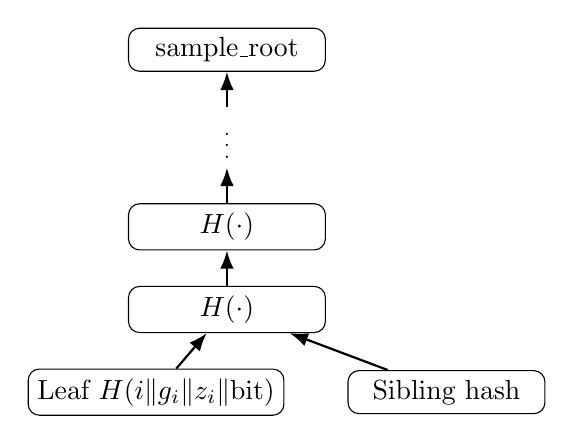
\begin{tikzpicture}[
    box/.style={draw, rounded corners, align=center, minimum width=2.5cm, minimum height=0.5cm},
    node distance=0.45cm and 0.8cm
  ]
  \node[box] (leafL) {Leaf $H(i \| g_i \| z_i \| \mathrm{bit})$};
  \node[box, right=of leafL] (leafR) {Sibling hash};
  \node[box, above=of leafL, xshift=0.9cm] (h1) {$H(\cdot)$};
  \node[box, above=of h1] (h2) {$H(\cdot)$};
  \node[above=of h2] (dots) {\scriptsize$\vdots$};
  \node[box, above=of dots] (root) {$\mathrm{sample\_root}$};

  \draw[-Latex, thick] (leafL) -- (h1);
  \draw[-Latex, thick] (leafR) -- (h1);
  \draw[-Latex, thick] (h1) -- (h2);
  \draw[-Latex, thick] (h2) -- (dots);
  \draw[-Latex, thick] (dots) -- (root);
  \end{tikzpicture}
  \caption{Merkle authentication path for a sampled trace element used as a proof witness.}
  \label{fig:merkle}
\end{figure}

\subsection{SP1 Proof Generation}
PP-Mark leverages the SP1 zkVM \cite{succinct2024sp1} to generate a standalone zero-knowledge proof receipt \(\pi\). The proof establishes, in zero knowledge, that the published binding value \(b\) and the committed sampled trace \(\mathcal{T}\), anchored by \(\mathrm{sample\_root}\), are consistent with a valid secret key \(k\) and payload \(\mathtt{bits}\), without revealing these secrets.

We adopt SP1 for engineering practicality: its Rust-based tooling and parallelizable proving architecture enable efficient integration into high-throughput generative pipelines. To reduce proving overhead, the circuit \(\mathcal{C}\) does not re-simulate the full latent embedding or inverse-CDF computation. Instead, it enforces only the minimal consistency constraints necessary to cryptographically bind the statistical detection parameters to the underlying secret state.

\subsubsection{Statement and Witness}
The SP1 proof \(\pi\) attests to the existence of a private witness \(w\) that satisfies the
verification predicate with respect to a public statement \(x\).

\begin{definition}
  \textbf{(Public Statement \(x\))}
  The public statement consists of the binding value \(b\), the commitment root
  \(\mathrm{sample\_root}\), the opening digest \(\mathrm{opening\_digest}\), the opening size
  \(k_{\mathrm{open}}\), and auxiliary verification metadata such as the Merkle tree depth.
  Other parameters, including the sampling size \(N\) and the LUT hash, are public for
  auditability but are not explicitly enforced within the circuit constraints.
\end{definition}

\begin{definition}
  \textbf{(Private Witness \(w\))}
The private witness contains sensitive generation data, including the secret key \(k\),
the Reed--Solomon codeword \(c\), and the sampled trace
\(\mathcal{T} = \{(i, g_i, z_i, \mathrm{bit})\}_{i \in S}\) together with the corresponding
Merkle authentication paths.
\end{definition}

\textbf{Circuit Constraints.}
The circuit \(\mathcal{C}\) enforces the core consistency relations of the system. In
particular, it verifies that the binding value is correctly computed as
\(b = \mathsf{H}(\texttt{"bind\_hash"} \,\|\, h_{\mathrm{ctx}} \,\|\, k)\), and that each
leaf in the sampled trace \(\mathcal{T}\) reconstructs the committed
\(\mathrm{sample\_root}\) via its Merkle authentication path. The circuit further enforces
that the trace \(\mathcal{T}\) is consistent with the deterministic sample set \(S\) and the
bit-mapping rule \(\mathrm{idx}(x,y)\) derived from \(b\). In addition, the circuit derives the opening positions from \(\mathrm{challenge\_seed}\), recomputes \(\mathrm{opening\_digest}\) from the corresponding trace entries, and enforces equality with the public digest.

The resulting receipt \(\pi\) is standalone and publicly verifiable. Since forging \(\pi\) is computationally infeasible without access to the secret key \(k\) and a valid sampled trace, the proof ensures that knowledge of the public detector alone is insufficient to fabricate valid provenance.

\subsection{Extraction and Verification}
Given an image, its associated metadata, and an SP1 receipt, the verifier performs DDIM
inversion to recover an approximate latent representation \(\hat{z}^{(0)}\). The verifier
computes a normalized image hash \(h_{\mathrm{img}}\), derives
\(\mathrm{challenge\_seed}\), and validates the opening subset \(K\) against the metadata
digest; this opening check is incorporated into
\(\text{VerifyReceipt}(\pi; x)\). The verifier then reconstructs \(m\), \(c\), and
\(\mathbf{bits}\) from the public binding value \(b\), regenerates the sample set \(S\), and
derives the expected sign pattern.

\begin{assumption}[Statistical Properties of Inversion Residuals]
\label{assum:noise}
Let \(\epsilon_i = \hat{z}_i - z_i\) denote the DDIM inversion residual at latent index \(i\).
We assume that \(\epsilon_i\) follows an approximately zero-mean distribution, i.e.,
\(\mathbb{E}[\epsilon_i] \approx 0\), and is weakly correlated with the watermark signal
\(s_i\).
\end{assumption}

Under Assumption~\ref{assum:noise}, the recovered residual \(r_i\) for each sampled index
\(i \in S\) is computed as
\begin{equation}
r_i
= \frac{\hat{z}_i - g_i}{\alpha_{\mathrm{eff}}}
= \frac{(z_i + \epsilon_i) - g_i}{\alpha_{\mathrm{eff}}}
= s_i + \frac{\epsilon_i}{\alpha_{\mathrm{eff}}}.
\label{eq:residual}
\end{equation}

PP-Mark uses \(N = 1000\) samples to compute the final detection score. This choice balances
statistical stability, reducing score variance through averaging, against the proving and
verification overhead of the SP1 pipeline. The detection score is defined as the normalized
correlation over the sample set \(S\):
\begin{equation}
\mathrm{score}
= \frac{|\langle r_S, s_S \rangle|}{\|s_S\| + \epsilon}.
\end{equation}

The score measures the alignment between the recovered residuals \(r_S\) and the expected
sign pattern \(s_S\). Finally, an image is accepted as authentic if and only if it satisfies
both the statistical and cryptographic verification criteria:

\begin{equation}
{\small
\text{Accept}(I,\pi)\iff (\mathrm{score}\ge\tau)\land(\text{VerifyReceipt}(\pi; x)=1).
}
\end{equation}


\begin{algorithm}[t]
\caption{Verify and Extract}
\label{alg:verify}
\begin{algorithmic}[1]
\STATE Input:
\parbox[t]{0.85\linewidth}{
image \(I\), metadata \(\mathrm{md}\) (including \(h_{\mathrm{ctx}}, b,
\mathrm{sample\_root}, \mathrm{opening\_digest}, k_{\mathrm{open}}\)), receipt \(\pi\)
}
\STATE \(\hat{z}^{(0)} \leftarrow \text{DDIM\_Inversion}(I)\)
\STATE Reconstruct \(\mathbf{bits}\) from \(b\); regenerate sample set \(S\) from \(c\)
\FOR{each \(i \in S\)}
  \STATE \(g_i \leftarrow F^{-1}(\mathsf{H}(\texttt{"u"} \,\|\, b \,\|\, i) \bmod 2^{32})\)
  \STATE \(r_i \leftarrow (\hat{z}_i - g_i) / \alpha_{\mathrm{eff}}\)
  \STATE \(s_i \leftarrow 2 \cdot \mathbf{bits}_{\mathrm{idx}(i)} - 1\)
\ENDFOR
\STATE \(\mathrm{score} \leftarrow \frac{|\langle r_S, s_S \rangle|}{\|s_S\| + \epsilon}\)
\STATE \(\texttt{proof\_ok} \leftarrow \text{VerifyReceipt}(\pi; \mathrm{md}, I)\)
\STATE Return \((\mathrm{score} \ge \tau) \land \texttt{proof\_ok}\)
\end{algorithmic}
\end{algorithm}

  
\subsection{Synchronization and Security Rationale}
To handle transformation-induced misalignment, PP-Mark employs an alignment search over
latent positions. A central efficiency--security trade-off arises from our use of
deterministic sampling with \(N=1000\), since verifying the full latent space within a ZKP
circuit would be computationally prohibitive for real-time deployment. Under bounded and
approximately independent samples, empirical averages concentrate in the Hoeffding sense
\cite{hoeffding1963}, enabling high-throughput verification while preserving the
statistical reliability required for stable detection.

Furthermore, the binding value \(b\) ties the watermark to the full generation context,
ensuring that any modification to the prompt or random seed induces a distinct
commitment. By anchoring statistical detection to a ZKP receipt \(\pi\), the detection
score becomes contingent on a valid cryptographic proof rather than on the score alone.
As a result, even if an adversary optimizes a forgery to achieve a high detection score,
verification fails in the absence of a consistent latent trace and proof, which cannot be
constructed without access to the secret witness.

\section{Experiments}
\subsection{Experimental Setup}
We use Stable Diffusion v2.1 base with a DDIM scheduler, 50 inference steps, and guidance scale 7.5. PP-Mark uses $\alpha=4.0$, sample count $N=1000$, and SHA-256 sampling for SP1. Prompts are drawn from the Stable-Diffusion-Prompts dataset. All methods are calibrated to the same 1\% FPR on clean(non-watermarked) images using their native detection statistics. We calibrate on clean SD2.1 images generated under the same settings.

\subsection{Imprint Forgery Attack}
Imprint forgery is a strong black-box and method-agnostic threat: from a
single watermarked reference image, an attacker attempts to transfer the watermark imprint onto an arbitrary cover so the verifier attributes it to the same source
\cite{muller2025blackbox}. This captures a realistic adversary who does not know the target watermark design but can adapt a proxy generator, making it a practical strong attack. We use SD2.1 for both the target and the proxy in the imprint-forgery attack. To evaluate this threat fairly, we construct a fixed prompt pool (200 prompts; 100/100 calibration/evaluation) and prepare a cover pool of 100 images as targets for attribution transfer. We fix 100 cover–reference pairs (one reference per cover) and reuse the same pairs across all methods to avoid pairing bias.

\subsubsection{Direct Imprint Forgery}
We apply the standard imprint-forgery optimizer to each fixed cover--reference pair and evaluate with each method’s native detector (Forgery Acceptance Rate(FAR)@1\%(False Positive Rate(FPR), $n=100$ per step).
Table~\ref{tab:direct-vulnerability} reports results for Tree-Ring and Gaussian Shading as a sanity check of the attack pipeline; both are highly vulnerable(TR: 0.92→0.97, GS: 1.00 across steps).


\sisetup{
  detect-weight=true,
  table-number-alignment=center,
  round-mode=places,
  round-precision=2
}

  \begin{table}[t]
    \caption{Direct vulnerability under targeted imprint forgery.
    FAR@1\%FPR (targeted verify); All methods evaluated at FPR=1\% (clean-calibrated)}
    \label{tab:direct-vulnerability}
    \begin{center}
      \begin{small}
        \begin{sc}
          \begin{tabular}{
          c
          S[table-format=1.3, round-mode=none] S[table-format=1.3, round-mode=none]
          }
            \toprule
            &
            \multicolumn{1}{c}{\textbf{TR}} &
            \multicolumn{1}{c}{\textbf{GS}} \\
            \cmidrule(lr){2-2}\cmidrule(lr){3-3}
            \textbf{Step}
            & {\textbf{FAR@1\%FPR}} & {\textbf{FAR@1\%FPR}} \\
            \midrule
            50 & 0.92 & 1.00 \\
            100 & 0.97 & 1.00 \\
            150 & 0.97 & 1.00 \\
            Avg. & 0.953 & 1.00 \\
            \bottomrule
          \end{tabular}
        \end{sc}
      \end{small}
    \end{center}
    \vskip -0.1in
  \end{table}

  \begin{table}[t]
      \caption{Transfer results by method and step.
      FAR@1\%FPR (targeted verify); All methods evaluated at FPR=1\% (clean-calibrated).}
      \label{tab:transfer-steps}
      \begin{center}
        \begin{small}
          \begin{sc}
            \resizebox{\linewidth}{!}{%
            \begin{tabular}{
            l c
            S[table-format=1.2] S[table-format=1.2]
            }
              \toprule
              & &
              \multicolumn{1}{c}{\textbf{TR}} &
              \multicolumn{1}{c}{\textbf{GS}} \\
              \cmidrule(lr){3-3}\cmidrule(lr){4-4}
              \textbf{Method} & \textbf{Step}
              & {\textbf{FAR@1\%FPR}} & {\textbf{FAR@1\%FPR}} \\
              \midrule

              \multirow{3}{*}{RingID} & 50 & 0.01 & 0.01 \\
                                        & 100 & 0.10 & 0.02 \\
                                        & 150 & 0.01 & 0.01 \\
                \addlinespace

                \multirow{3}{*}{StableSig} & 50 & 0.04 & 0.01 \\
                                           & 100 & 0.04 & 0.02 \\
                                           & 150 & 0.02 & 0.02 \\
                \addlinespace

                \multirow{3}{*}{HiDDeN} & 50 & 0.04 & 0.01 \\
                                        & 100 & 0.02 & 0.03 \\
                                        & 150 & 0.01 & 0.03 \\
                \addlinespace

                \multirow{3}{*}{WIND} & 50 & 0.01 & 0.01 \\
                                     & 100 & 0.01 & 0.01 \\
                                     & 150 & 0.01 & 0.01 \\
                \addlinespace

                \multirow{3}{*}{PP-Mark${\mathrm{score}}$} & 50 & 0.00 & 0.00 \\
                                         & 100 & 0.00 & 0.01 \\
                                         & 150 & 0.01 & 0.01 \\
                \addlinespace

                \multirow{3}{*}{PP-Mark${\mathrm{accept}}$} & 50 & 0.00 & 0.00 \\
                                         & 100 & 0.00 & 0.00 \\
                                         & 150 & 0.00 & 0.00 \\

              \bottomrule
            \end{tabular}}
          \end{sc}
        \end{small}
      \end{center}
      \vskip -0.1in
    \end{table}



\begin{table*}[t]
    \caption{Transfer summary over steps.
    FAR@1\%FPR (targeted verify) with 95\% CI.
    All methods evaluated at FPR=1\% (clean-calibrated).
    $\Delta$\% is computed as $(k-k_{\mathrm{PP-Markscore}})/k_{\mathrm{PP-Markscore}} \times 100$, where $k_{\mathrm{PP-Markscore}}=1$ (TR) and $k_{\mathrm{PP-Markscore}}=2$ (GS). Fisher $p$ is from a one-sided Fisher exact test vs PP-Mark${\mathrm{score}}$ (H1: method $>$ PP-Mark${\mathrm{score}}$).}
    \label{tab:transfer-summary}
    \begin{center}
      {\scriptsize
      \setlength{\tabcolsep}{2pt}
      \renewcommand{\arraystretch}{1}
        \begin{sc}
          
          \begin{tabular}{
          l
          S[table-format=1.4, round-mode=places, round-precision=4, round-pad=true] c c c
          S[table-format=1.4, round-mode=places, round-precision=4, round-pad=true] c c c
          }
            \toprule
            & \multicolumn{4}{c}{\textbf{TR}} & \multicolumn{4}{c}{\textbf{GS}} \\
            \cmidrule(lr){2-5}\cmidrule(lr){6-9}
            \textbf{Method} & {\textbf{FAR@1\%FPR}} & \textbf{95\% CI} & \textbf{$\Delta$\%} &
  \textbf{Fisher $p$}
            & {\textbf{FAR@1\%FPR}} & \textbf{95\% CI} & \textbf{$\Delta$\%} & \textbf{Fisher $p$} \\
            \midrule
            RingID & 0.0400 & 0.0208--0.0688 & +1100.0 & 0.0016 & 0.0133 & 0.0036--0.0338 & +100.0 &
  0.3430 \\
            StableSig & 0.0333 & 0.0161--0.0604 & +900.0 & 0.0055 & 0.0167 & 0.0054--0.0385 & +150.0 &
  0.2252 \\
            HiDDeN & 0.0233 & 0.0094--0.0475 & +600.0 & 0.0343 & 0.0233 & 0.0094--0.0475 & +250.0 & 0.0882
  \\        WIND & 0.0100 & 0.0021--0.0289 & +200.0 & 0.3119 & 0.0100 & 0.0021--0.0289 & +50.0 & 0.5000 \\
            PP-Mark${\mathrm{score}}$ & 0.0033 & 0.0001--0.0184 & -- & -- & 0.0067 & 0.0008--0.0239 & -- & -- \\
            PP-Mark${\mathrm{accept}}$ & 0.0000 & -- & -- & -- & 0.0000 & -- & -- & -- \\            
            \bottomrule
          \end{tabular}
        \end{sc}
      }
    \end{center}
    \vskip -0.1in
  \end{table*}
  
  \subsubsection{Transfer Imprint Forgery} 
  We evaluate cross-method vulnerability to the standard imprint-forgery pipeline. Tree-Ring (TR) and Gaussian Shading (GS) are used as canonical imprint sources to keep the attack fixed across methods. For each fixed cover--reference pair, we extract the imprint from a single TR/GS-watermarked reference and optimize it onto the cover. All detectors are evaluated under thresholds calibrated to 1\% FPR on clean images, so differences reflect detector susceptibility under the same fixed pairings and step budget.(PP‑Mark$_{\mathrm{score}}$ reports score-only acceptance for cross-method comparability, while PP‑Mark$_{\mathrm{accept}}$ enforces the full verification rule.)
  
  Table~\ref{tab:transfer-steps} reports step-wise transfer success for each method when the imprint source is TR or GS. PP‑Mark$_{\mathrm{score}}$ remains at 0.00--0.01 across steps, indicating that the standard imprint-forgery pipeline rarely pushes it beyond its calibrated false-positive floor. In contrast, RingID/StableSignature/HiDDeN exceed this floor, showing materially higher susceptibility under identical calibration and attack conditions. 
  
  \subsubsection{Summary of Transfer Imprint Forgery}
Table~\ref{tab:transfer-summary} summarizes transfer acceptance rates aggregated across the three optimization steps under a fixed pairing protocol. Across both TR- and GS-sourced imprints, PP‑Mark$_{\mathrm{score}}$ consistently attains the lowest acceptance rates, effectively remaining at or below the 1\% calibration floor (0.0033 for TR and 0.0067 for GS). This indicates that the imprint-forgery attack fails to move PP-Mark’s score beyond the statistical noise floor of a clean image. In contrast, RingID, Stable Signature, and HiDDeN exhibit substantially higher transfer acceptance under TR-sourced attacks, with point estimates an order of magnitude larger than PP‑Mark$_{\mathrm{score}}$. 

The $\Delta\%$ column reports ratios computed from raw counts relative to PP‑Mark$_{\mathrm{score}}$’s small denominators. While these ratios appear numerically large, they are intended as descriptive summaries rather than primary effect size. The absolute FARs and their $95\%$ confidence intervals therefore provide the appropriate basis for comparison and consistently rank PP‑Mark$_{\mathrm{score}}$ as the least susceptible method under the same calibration and attack conditions. 

One-sided Fisher exact tests against PP‑Mark$_{\mathrm{score}}$ further support this ordering for TR-sourced imprints: the higher acceptance rates of RingID, Stable Signature, and HiDDeN are statistically significant ($p=0.0016$, $0.0055$, and $0.0343$, respectively). For GS-sourced imprints, the differences do not reach statistical significance at the $0.05$ level. Nevertheless, the point estimates and confidence intervals preserve the same practical ordering, with PP‑Mark$_{\mathrm{score}}$ remaining the least vulnerable among all evaluated methods.

\begin{figure}[t]
    \centering
    \includegraphics[width=1\linewidth]{transfer forest(WIND).pdf}
    \caption{Cross‑method transfer at FPR=1\%. Error bars denote 95\% CI; the vertical line indicates PP‑MarkPP-Mark${\mathrm{score}}$.}
    \label{fig:transfer-forest}
\end{figure}

\subsection{White-Box Forgery Attack}
We consider a strongest case white-box adversary with full access to each detector and
gradients, optimizing inputs to maximize the detection score under an $\ell_\infty$ budget $\epsilon=2/255$ using $T=150$ PGD steps. For each method, forgery acceptance is defined by $\mathrm{score}\ge\tau$, where $\tau$ is calibrated at 1\% FPR. In contrast, PP‑Mark$_{\mathrm{accept}}$ requires passing both statistical and cryptographic checks. 

All methods are attacked via their differentiable pipelines: Stable Signature and HiDDeN use differentiable decoders; RingID and PP‑Mark$_{\mathrm{score}}$ use differentiable inversion-based scores. For WIND, we optimize a differentiable Fourier-distance surrogate while evaluating against the actual detector. 

Table~\ref{tab:white-box-summary} shows outcomes across methods. Most baselines reach FAR@1\%FPR = 1.00, while PP-Mark$_{\mathrm{score}}$ remains lower (0.76).  PP‑Mark$_{\mathrm{score}}$ attains a lower FAR but a smaller mean step among accepted cases
than WIND. This is consistent with the objective structure: PP‑Mark uses a keyed, image‑conditioned correlation/bit‑sign score (sample indices and sign map vary per image), which can yield highly variable progress, some images align quickly while others stall. WIND uses a fixed pattern/mask reconstruction objective shared across images, which promotes more uniform progress and thus more consistent acceptance, typically at later steps on average. Thus, PP‑Mark’s faster successes reflect higher variance rather than overall weakness, whereas WIND trades slightly slower convergence for near‑certain acceptance. Figure~\ref{fig:wb_forge_far_curves} shows the cumulative FAR trajectories across steps. 
  
\begin{table}[t]
  \caption{White-Box forgery outcomes across methods. FAR@1\%FPR is the forgery acceptance rate. Avg.\ Steps to FA reports, among forgery acceptances, the mean optimization step (within a fixed budget of 150 steps) at which $\mathrm{score}\ge\tau$ first occurs. PSNR is averaged against the original cover image.}
  \label{tab:white-box-summary}
  \begin{center}
    {\footnotesize
    \setlength{\tabcolsep}{2pt}
    \renewcommand{\arraystretch}{1}
      \begin{sc}
        \begingroup
        \hypersetup{hidelinks}
        \begin{tabular}{
          l
          S[table-format=1.2, round-mode=places, round-precision=2, round-pad=true]
          S[table-format=3.2, round-mode=places, round-precision=2, round-pad=true]
          S[table-format=2.2, round-mode=places, round-precision=2, round-pad=true]
        }
          \toprule
          \textbf{Method}
          & {\makecell{\textbf{FAR}\\ \textbf{@1\%FPR}}}
          & {\makecell{\textbf{Avg.\ }\\ \textbf{Steps to FA}}}
          & {\makecell{\textbf{Avg.\ }\\ \textbf{PSNR $\uparrow$}}} \\
          \midrule
          StableSig                 & 1.00 & 5.40  & 65.91 \\
          HiDDeN                    & 1.00 & 8.08  & 62.96 \\
          RingID                    & 1.00 & 2.26  & 74.51 \\
          WIND                      & 1.00 & 22.20 & 55.76 \\
          PP-Mark$_{\mathrm{score}}$  & 0.76 & 17.42 & 67.69 \\
          PP-Mark$_{\mathrm{accept}}$ & 0.00 & \multicolumn{1}{c}{--} & \multicolumn{1}{c}{--} \\          \bottomrule
        \end{tabular}
        \endgroup
      \end{sc}
    }
  \end{center}
  \vskip -0.1in
\end{table}

\begin{figure}[H]
    \centering
    \includegraphics[width=1\linewidth]{wb_forge_far_curves.pdf}
    \caption{Cumulative FAR@1\%FPR vs. optimization step for all methods under the same attack budget and evaluation setup.}
    \label{fig:wb_forge_far_curves}
\end{figure}

For PP-Mark$_{\mathrm{accept}}$, watermark acceptance requires proof verification. The
attacked image changes the image hash $h_{\mathrm{img}}$, which changes 
$\mathrm{challenge\_seed}$ and thus the opening positions and the recomputed 
$\mathrm{opening\_digest}$. As a result, the verifier’s opening check and proof verification fails, PP‑Mark$_{\mathrm{accept}}$ stays at FAR=0.

\subsection{Removal Attacks}
We assess PP-Mark’s resilience to watermark erasure at a fixed detection threshold (FPR=1\%), focusing on whether signals can be removed without compromising image quality.

\subsubsection{Regeneration Attack}
The adversary employs diffusion-based re-synthesis to wash out the watermark while preserving visual content \cite{zhao2024removable}. PP-Mark remains highly detectable at all noise steps (TPR 0.98), whereas StableSig and HiDDeN drop to 0.01–0.06. We evaluate survival rates across varying noise intensities; detailed configurations and per-step results are provided in in Appendix~\ref{sec:Regeneration Attack}. 

\subsubsection{Steganalysis Attack}
This attack estimates and subtracts the watermark signal using $K$ reference samples. PP-Mark stays highly detectable as K increases (TPR 0.864–0.963), whereas Tree-Ring drops to 0.02–0.038 and StableSig stays around 0.17–0.20. Full results for various $K$ are detailed in Appendix~\ref{Steganalysis Attack}.

\subsection{Image Transformations}
We report post-attack detection on the standard set; detailed settings and results are provided in Appendix~\ref{Image Transformations}.

\subsection{Generation Distributional Fidelity}
We assess distributional fidelity using KID (an unbiased metric) between clean and watermarked image sets; full results are provided in Appendix~\ref{Generation Distributional Fidelity}.

\section{Limitations} 
While PP-Mark demonstrates superior resistance to imprint forgery than baselines and remains robust against various removal attacks, its decentralized verification relies on ZKP. Generating and verifying these proofs adds computational, storage, and bandwidth overhead that scales with the sample count $N$, which can impact system throughput(in Appendix). Furthermore, the system assumes the generator’s secret witness remains secure. If the secret is compromised, an attacker can mint valid receipts and produce verified forgeries under the victim’s identity, effectively breaking provenance. Additional limitations and discussions are continued in Appendix~\ref{Additional Limitations and Dicussions}.

\section{Conclusion}
PP-Mark leverages public zero-knowledge proof to enable decentralized verification of AI-generated provenance, while substantially reducing susceptibility to forgery attack. By anchoring the context-bound detection score to a publicly verifiable cryptographic proof, PP-Mark demonstrates that decentralized, open verification can coexist with robust resistance to state-of-the-art forgery attack. We hope this work lays a foundation for transparent and robust provenance verification of AI-generated content.

\section*{Impact Statement}
This work provides a decentralized, verifiable mechanism for AI image provenance, helping reduce misattribution and synthetic media misuse. By removing reliance on centralized APIs and addressing forgery threats, PP-Mark enables transparent auditing of provenance claims under clear operational assumptions. We view this as a technical building block that complements broader socio-technical efforts for the responsible deployment of generative AI.


% In the unusual situation where you want a paper to appear in the
% references without citing it in the main text, use \nocite
\nocite{langley00}

\bibliography{example_paper}
\bibliographystyle{icml2026}

%%%%%%%%%%%%%%%%%%%%%%%%%%%%%%%%%%%%%%%%%%%%%%%%%%%%%%%%%%%%%%%%%%%%%%%%%%%%%%%
%%%%%%%%%%%%%%%%%%%%%%%%%%%%%%%%%%%%%%%%%%%%%%%%%%%%%%%%%%%%%%%%%%%%%%%%%%%%%%%
% APPENDIX
%%%%%%%%%%%%%%%%%%%%%%%%%%%%%%%%%%%%%%%%%%%%%%%%%%%%%%%%%%%%%%%%%%%%%%%%%%%%%%%
%%%%%%%%%%%%%%%%%%%%%%%%%%%%%%%%%%%%%%%%%%%%%%%%%%%%%%%%%%%%%%%%%%%%%%%%%%%%%%%

\clearpage

\appendix
\section{Ablation Study}
\subsection{Sample Size and Statistical Reliability}
We analyze the trade-off between statistical reliability and computational overhead by varying the number of sampled latent positions $N \in \{200, \dots, 1500\}$. We identify $N=1000$ as the reasonable point where statistical stability is maximized without incurring excessive prover latency or bandwidth costs.

\textbf{Statistical Concentration:} Theoretically, the detection score (cosine similarity) acts as a smooth function of bounded aggregates, suggesting Hoeffding-sense concentration. Empirically, the score's standard deviation across images decreases by 7.7\% as $N$ increases from 200 to 1000 ($0.1409 \rightarrow 0.1301$). However, increasing $N$ further to 1500 yields only a marginal 3.0\% additional reduction, indicating diminishing returns in variance reduction. 

  \begin{figure}[H]
      \centering
      \includegraphics[width=0.9\linewidth]{score_std_vs_n_grid.pdf}
      \caption{Score concentration: standard deviation vs.\ sample count $N$.}
      \label{fig:score-std-n}
  \end{figure}
  
  \begin{figure}[H]
      \centering
      \includegraphics[width=0.9\linewidth]{knee_tradeoff_plot.pdf}
      \caption{Knee trade-off between proving cost and score variability.}
      \label{fig:knee-tradeoff}
  \end{figure}
  
\textbf{Computational Cost:} On a single H100 GPU for proving (CPU for verification), SP1 prover and verification times scale approximately linearly with $N$. Proving time rises from 32.3s ($N=200$) to 48.6s ($N=1000$), with verification following a similar trend.  Figure~\ref{fig:sp1-vs-risc0-timing} shows that SP1 is faster in this setting because its prover is optimized for GPU throughput and parallel execution of the trace, while the RISC0 path here uses a heavier zkVM stack and a CPU-bound proving workflow. 

  \begin{table}[H]
    \caption{SP1 prove/verify timing vs.\ sample count $N$ (GPU prove, CPU verify).}
    \label{tab:sp1-k-sweep-timing}
    \begin{center}
      \begin{small}
        \begin{sc}
          \begin{tabular}{c S[table-format=2.3] S[table-format=1.3]}
            \toprule
            \textbf{N} & {\textbf{Prove (s)}} & {\textbf{Verify (s)}} \\
            \midrule
            200  & 32.309 & 4.468 \\
            400  & 38.278 & 5.640 \\
            600  & 39.932 & 5.886 \\
            800  & 43.465 & 6.651 \\
            1000 & 48.572 & 7.589 \\
            1200 & 49.425 & 8.877 \\
            1500 & 60.272 & 9.802 \\
            \bottomrule
          \end{tabular}
        \end{sc}
      \end{small}
    \end{center}
    \vskip -0.1in
  \end{table}

\begin{figure}[H]
  \centering
  \includegraphics[width=0.9\linewidth, trim=0 0 0 25pt, clip]{sp1_vs_risc0_k1000_timing.pdf}
  \caption{Prover and verifier timings at $N=1000$ ($\alpha=4.0$). SP1 uses a single H100 GPU for proving with CPU receipt verification; RISC0 uses the same SD2.1 setup and public inputs with CPU receipt verification.}
  \label{fig:sp1-vs-risc0-timing}
\end{figure}
 


\subsection{Watermark Strength}
We study the effect of watermark strength $\alpha$ on visual quality while fixing the sampling budget at $N=1000$. We report BRISQUE (lower is better) and focus on the 95th percentile across images to capture tail behavior. For each $\alpha \in \{3.0, 3.5, 4.0, 4.5\}$ we evaluate 100 watermarked images under identical settings. 

The BRISQUE p95 is relatively stable from $\alpha=3.0$ to $4.0$ (roughly $34.1$--$34.9$), but it jumps at $\alpha=4.5$ to $40.5$, indicating a heavier quality tail. This suggests that pushing $\alpha$ beyond 4.0 yields a disproportionate increase in worst-case artifacts without a clear compensating gain in reliability, given that $N=1000$ already stabilizes detection. We therefore select $\alpha=4.0$ as a conservative balance between robustness and perceptual quality (Fig.~\ref{fig:alpha-brisque-p95}).

\begin{figure}[H]
    \centering
    \includegraphics[width=0.9\linewidth]{alpha_brisque_p95.pdf}
    \caption{BRISQUE p95 vs.\ watermark strength $\alpha$ (lower is better).}
    \label{fig:alpha-brisque-p95}
\end{figure}


\section{Regeneration Attack}\label{sec:Regeneration Attack}
We evaluate detection rates after regeneration at each noise level to measure how well the watermark survives re-synthesis. Table~\ref{tab:zhao-regen-full100} reports detection rates after regeneration.
  \begin{table}[H]
    \caption{Post-Regeneration attack detection rate at FPR=1\% thresholds; each noise step uses 100 images; noise step is 30/60/100.}
    \label{tab:zhao-regen-full100}
    \begin{center}
      \begin{small}
        \begin{sc}
          \begin{tabular}{
          l
          S[table-format=2.0]
          S[table-format=2.0]
          S[table-format=2.0]
          }
            \toprule
            & \multicolumn{3}{c}{\textbf{Noise step}} \\
            \cmidrule(lr){2-4}
            \textbf{Method} & \multicolumn{1}{c}{\textbf{30steps}} & \multicolumn{1}{c}{\textbf{60steps}}
              & \multicolumn{1}{c}{\textbf{100steps}} \\
            \midrule
            StableSig & 0.04 & 0.02 & 0.03 \\
            HiDDeN & 0.010 & 0.06 & 0.04 \\
            Tree-Ring & 0.95 & 0.93 & 0.93 \\
            PP-Mark & 0.98 & 0.98 & 0.98 \\
            \bottomrule
          \end{tabular}
        \end{sc}
      \end{small}
    \end{center}
    \vskip -0.1in
  \end{table}


\begin{table}[H]
  \caption{Steganalysis removal summary (TPR@1\%FPR) by K.} 
  \label{tab:steg-removal-summary}
  \begin{center}
    \begin{small}
      \begin{sc}
        \sisetup{detect-all, mode=text}
        \setlength{\tabcolsep}{8pt} % 열 사이 간격을 가독성 좋게 조절
        \renewcommand{\arraystretch}{1.1}
        \begin{tabular}{
          l 
          c % K 열: S 대신 c를 사용하여 소수점 없이 정수 그대로 가운데 정렬
          S[table-format=1.3, round-mode=places, round-precision=3]
          S[table-format=2.2, round-mode=places, round-precision=2]
        }
          \toprule
          \textbf{Method} & \textbf{K} & \textbf{TPR@1\%FPR} \\
          \midrule
          \multirow{4}{*}{StableSig}
            & 10   & 0.200 \\
            & 100  & 0.200 \\
            & 500  & 0.173 \\
            & 1000 & 0.171 \\
          \midrule
          \multirow{4}{*}{Tree-Ring}
            & 10   & 0.190 \\
            & 100  & 0.020 \\
            & 500  & 0.038 \\
            & 1000 & 0.035 \\
          \midrule
          \multirow{4}{*}{WIND}
            & 10   & 1.000 & \\
            & 100  & 1.000 & \\
            & 500  & 1.000 & \\
            & 1000 & 1.000 & \\
          \midrule
          \multirow{4}{*}{PP-Mark}
            & 10   & 0.864 & \\
            & 100  & 0.959 & \\
            & 500  & 0.963 & \\
            & 1000 & 0.958 & \\
          \bottomrule
        \end{tabular}
      \end{sc}
    \end{small}
  \end{center}
  \vskip -0.1in
\end{table}
\section{Steganalysis Attack} \label{Steganalysis Attack}
We sweep K={10, 100, 500, 1000} and evaluate the post-attack detection rate at the calibrated FPR=1\% threshold. Table~\ref{tab:steg-removal-summary} shows that StableSignature and Tree-Ring detection drops as K increases, indicating increasing removal effectiveness, while PP-Mark remains highly detectable even at large K.




\section{SPSA-based Removal Attack}
We consider a targeted removal adversary that, given a watermarked image $x_w$ and its
correct binding $b$, directly minimizes the public verifier’s score using SPSA. The score is the same correlation used by the verifier, with $S$ and $s_S(b)$ reconstructed from metadata . 
We trace steps $0,5,10,\dots,50$ fixing $\tau$ to the clean FPR=1\% threshold. The trace shows that the score drops below $\tau$ early, the visual quality collapses immediately (PSNR $\approx 4.7$–$6.9$ across steps 5–50). Thus, removal is possible only under destructive distortions; when a quality constraint (e.g., PSNR $\ge 30$) is enforced, no valid outputs are obtained.

  \begin{figure}[H]
    \centering
    \includegraphics[width=0.9\linewidth, trim=0 0 0 25pt, clip]{imprint_removal_step5_split.pdf}
    \caption{PP-Mark removal trace. top: score vs step with \(\tau\) (clean FPR=1\%); bottom: PSNR vs step with the PSNR=30 reference line.}
    \label{fig:imprint-removal-step5}
  \end{figure}

\begin{figure}[H]
    \centering
    \begin{subfigure}[t]{0.48\linewidth}
        \centering
        \includegraphics[width=\linewidth]{before_imprint_romoval.undefined.pdf}
        \caption*{(a) Original Watermarked Image}
    \end{subfigure}
    \hfill
    \begin{subfigure}[t]{0.48\linewidth}
        \centering
        \includegraphics[width=\linewidth]{after_imprint_romoval50.undefined.pdf}
        \caption*{(b) After Removal Attack}
    \end{subfigure}
    \vspace{0.6em}
    \caption{(a) A watermarked image. (b) The result of an SPSA-based removal attack, fidelity loss (PSNR $\approx$ 7.36).} 
    \label{fig:visual-breakdown}
\end{figure}
  

\section{SPSA-based Forgery Attack}
We study an adaptive adversary that, given a cover image $x_c$ and its target metadata $b$, attempts to directly maximize the verifier’s score. In this setup, the oracle is the PP-Mark verifier, and $b$ denotes the specific metadata/proof pair for a fixed target. The adversary performs DDIM inversion to obtain $\hat{z}^{(0)}$ and solves 

  \begin{equation}
  \max_{\delta}\; \mathrm{score}\!\left(G(\hat{z}^{(0)} + \delta), b\right)
  \label{eq:adaptive_max}
  \end{equation}

where $G(\cdot)$ is the diffusion decoder and $\mathrm{score}(\cdot)$ is the correlation computed against $b$. A gradient-free SPSA loop \cite{spall1992spsa} to estimate the optimization landscape through black-box score queries. The adversary is unable to push the forged image's score above the calibrated threshold $\tau$. The SPSA-based optimization fails to find a viable path to raise the score; instead, it merely introduces visual degradation.

Figure~\ref{fig:adaptive-score-hist-per-image} plots the PP-Mark score distributions across optimization steps under instance-specific targeting where each image uses its
own metadata/proof. The dashed line indicates the calibrated threshold $\tau$. Across steps, most scores remain below $\tau$, with only a small tail crossing the boundary. 

Table~\ref{tab:adaptive-instance} summarizes the attack. Even though the attacker optimizes the exact verification score using the target metadata for each instance, the targeted acceptance remains low. 

\begin{table}[H]
    \caption{PP-Mark under SPSA Targeting. PSNR is a mean value computed against the original cover image.}
    \label{tab:adaptive-instance}
    \begin{center}
      \begin{small}
        \begin{sc}
          \begin{tabular}{
          c
          S[table-format=1.3, round-mode=none] S[table-format=1.2]
          }
            \toprule
            \textbf{Step}
            & {\textbf{FAR@1\%FPR}} & {\textbf{PSNR$\uparrow$}} \\
            \midrule
            50 & 0.02 & 6.55 \\
            100 & 0.00 & 6.61 \\
            150 & 0.01 & 6.63 \\
            Avg. & 0.01 & 6.60 \\
            \bottomrule
          \end{tabular}
        \end{sc}
      \end{small}
    \end{center}
    \vskip -0.1in
  \end{table} 
  
  \begin{figure}[H]
    \centering
    \includegraphics[width=0.9\linewidth, trim=0 0 0 35pt, clip]{(instance specific)Adaptive attack Histogram-1.pdf}
    \caption{PP-Mark score distribution by step. The dashed line marks $\tau$ (clean FPR=1\%).}
    \label{fig:adaptive-score-hist-per-image}
  \end{figure} 


  



\section{Additional Limitations and Dicussions}\label{Additional Limitations and Dicussions}
\textbf{Image Rotation}
Among the image transformations evaluated, rotation emerged as the most vulnerable: 60\% at $30^\circ$, 24\% at $45^\circ$, and 10\% at $50^\circ$. Since PP-Mark targets anti-forgery verification rather than full geometric invariance, small rotations or orientation normalization in practice may limit the impact on same-image recognition; however, the sharp drop under deliberate rotations indicates a structural limitation, likely because rotation resampling/interpolation disrupts the phase/sign of the high-frequency watermark pattern. Explicit alignment or rotation-invariant scoring would be needed to address this. 

\textbf{Reliance on Explicit Proof Artifacts}
A fundamental shift in PP-Mark is the transition from implicit verification to explicit proof reliance. Traditional diffusion watermarking schemes, such as TreeRing, operate under an implicit model where a proprietary verifier (a private API or internal model) acts as a hidden oracle. In these centralized frameworks, the image is the only required public artifact because the trust is encapsulated within the verifier's private infrastructure.

PP-Mark, by contrast, removes this private infrastructure to enable decentralized, public auditing. This design necessitates an explicit proof artifact which must be available to the verifier to reproduce the provenance claim. This creates a structural reliance:

\textbf{Decentralization Trade-off:} While removing the trust bottleneck of a central API, the system now requires the persistence of the proof alongside the content. The proof is not a leak of the secret, but a necessary, standalone witness of the generation context.

\textbf{Verification Failure Modes:} If this proof or other artifact is detached, deleted, or corrupted, the image may reverts to an unverified state, even if the underlying latent traces remain intact. This proof-dependency means that the reliability of provenance is bound to the availability of the cryptographic receipt.

To harden the system against artifacts loss or targeted attack, future work should focus on anchoring verification artifacts into decentralized infrastructures:

\textbf{Immutable Integrity via IPFS:} By utilizing decentralized storage like IPFS, the ZKP artifacts can be managed through content-addressing. Instead of relying on a fragile URL or local file path, the proof is identified by its cryptographic hash (CID). This ensures integrity; because the CID changes if the proof is altered, any successfully retrieved artifact is mathematically guaranteed to be the original, untampered witness generated at the time of creation. 

\textbf{Availability and Retrieval:} Anchoring these CIDs on a public blockchain or a distributed ledger provides a permanent, time-stamped registry of provenance. This setup enables robust retrieval; even if the original generator’s server goes offline or the image's external metadata is stripped, a verifier can use a pointer (such as a hash of the image itself or a small embedded ID) to query the ledger and recover the corresponding ZKP artifacts. 

\section{Image Transformations} \label{Image Transformations}
  Image Transformations experiments measured watermark detection accuracy after each transformation (post-
  attack detection rate; score$\geq\tau$, FPR=1\%). Detection rates remained high for most transforms:
  random crop + resize (keep ratio=0.75) 70\%, JPEG q25 94\%, blur $8\times 8$ 100\%, noise ($\sigma=0.1$)
  86\%, brightness jitter (0.6) 98\%. 

\section{Generation Distributional Fidelity}\label{Generation Distributional Fidelity}
Table~\ref{tab:kid-500} reports KID \cite{binkowski2018mmdgan} using a moderate subset (500) with multiple splits, which yields a stable estimate. Checks with smaller (subset=100) and larger (subset=1000) subsets give similar values, indicating that the result is not sensitive to subset size. The low KID indicates that the distribution of watermarked images remains close to the clean reference image distribution, suggesting minimal distributional shift due to watermarking.

\begin{figure}[H]
    \centering
    \begin{subfigure}[t]{0.48\linewidth}
      \centering
      \includegraphics[width=\linewidth]{ppmark_watermarked1.pdf}
      \caption*{}
    \end{subfigure}
    \hfill
    \begin{subfigure}[t]{0.48\linewidth}
      \centering
      \includegraphics[width=\linewidth]{ppmark_watermarked2.pdf}
      \caption*{}
    \end{subfigure}

    \vspace{0.6em}

    \begin{subfigure}[t]{0.48\linewidth}
      \centering
      \includegraphics[width=\linewidth]{ppmark_watermarked3.pdf}
      \caption*{}
    \end{subfigure}
    \hfill
    \begin{subfigure}[t]{0.48\linewidth}
      \centering
      \includegraphics[width=\linewidth]{ppmark_watermarked4.pdf}
      \caption*{}
    \end{subfigure}

    \caption{Examples of PP-Mark watermarked images}
    \label{fig:alpha4-qual}
\end{figure}

\newpage

\begin{table}[H]
    \caption{KID for generation distributional fidelity (subset=500, splits=20).}
    \label{tab:kid-500}
    \begin{center}
      \begin{small}
        \begin{sc}
          \begin{tabular}{
          c
          S[
            table-format=1.7,
            round-mode=places,
            round-precision=7,
            group-digits=false
          ]
          }
            \toprule
            \textbf{Subset} & {\textbf{KID}} \\
            \midrule
            500 & 0.0011014 \\
            \bottomrule
          \end{tabular}
        \end{sc}
      \end{small}
    \end{center}
    \vskip -0.1in
\end{table}


  









  
  
%%%%%%%%%%%%%%%%%%%%%%%%%%%%%%%%%%%%%%%%%%%%%%%%%%%%%%%%%%%%%%%%%%%%%%%%%%%%%%%
%%%%%%%%%%%%%%%%%%%%%%%%%%%%%%%%%%%%%%%%%%%%%%%%%%%%%%%%%%%%%%%%%%%%%%%%%%%%%%%

\end{document}

% This document was modified from the file originally made available by
% Pat Langley and Andrea Danyluk for ICML-2K. This version was created
% by Iain Murray in 2018, and modified by Alexandre Bouchard in
% 2019 and 2021 and by Csaba Szepesvari, Gang Niu and Sivan Sabato in 2022.
% Modified again in 2023 and 2024 by Sivan Sabato and Jonathan Scarlett.
% Previous contributors include Dan Roy, Lise Getoor and Tobias
% Scheffer, which was slightly modified from the 2010 version by
% Thorsten Joachims & Johannes Fuernkranz, slightly modified from the
% 2009 version by Kiri Wagstaff and Sam Roweis's 2008 version, which is
% slightly modified from Prasad Tadepalli's 2007 version which is a
% lightly changed version of the previous year's version by Andrew
% Moore, which was in turn edited from those of Kristian Kersting and
% Codrina Lauth. Alex Smola contributed to the algorithmic style files.
